\section{experimental evaluation}\label{sec:exp}
In this section, we conduct extensive experiments by comparing the proposed hash table design \voter with several state-of-the-art approaches for GPU-based hash tables. 
Section~\ref{sec:exp:setup} introduces the experimental setup. 
Sections~\ref{sec:exp:tune}, \ref{sec:exp:static} and \ref{sec:exp:dynamic} presents the discussions on the sensitivity analysis of \voter, the static and the dynamic experiments respectively.

\subsection{Experiment Setup}\label{sec:exp:setup}

\vspace{1mm}\noindent\textbf{Baselines.} We compare \voter with several state-of-the-art hash table implementations on GPUs. which are listed as the following:
\begin{itemize}
	\item \cudpp is a popular CUDA primitive library\footnote{https://github.com/cudpp/cudpp} which contains the cuckoo hash table implementation published in~\cite{alcantara2009real}. 
	For \cudpp, each hash value stores only one KV pair with 64 bits size (32 bits for key and 32 bits for value). 
	\cudpp only supports \formal{insert} and \formal{find} operations. We use the default setup of \cudpp with three hash functions. \yc{how many exactly?}
	\item \megakv is a warp-centric approach for GPU-based key value store published in~\cite{zhang2015mega}. \megakv employs a cuckoo hash with two hash functions and
	it allocates a bucket for each hash value. However, it does not lock a bucket when performing update. Instead, it uses intra-block synchronization to resolve race condition. 
	\item \slab is a state-of-the-art GPU-based dynamic hash table \cite{ashkiani2018dynamic}, which employs chaining and dedicated memory allocator for resizing.
	%\item \google is an efficient CPU-based hash table implementation\footnote{https://github.com/sparsehash/sparsehash-c11/}. We choose the \emph{dense\_hash\_map} implementation since it provides the best efficiency.
	\item \voter is the approach proposed in this paper.
\end{itemize}
We adopt the original implementations of the compared baselines from their corresponding inventors. 
%For \megakv, we note that its intra-block synchronization could lead to inconsistency issue as well as a large number of insertion failures, especially when the filled factor is high.  
%Thus, we revise its code by replacing the intra-block synchronization with atomicExch to resolve the race condition. The adoption of atomicExch preserves the design principle of \megakv for \emph{not} locking the entire bucket for updates. Moreover, it leads to less insertion failures and similar performance against its original implementation. 

%Note that we do not compare with the dynamic GPU hash approach proposed in \cite{ashkiani2018dynamic} for two major reasons. First, we cannot obtain the original implementation from its authors. Second, the approach devises a dedicated memory allocator other than cudaMalloc. A dedicated allocator will improve the performance but add complexity the system. Additionally, it needs to occupy a large memory in advance and is not transparent to other GPU applications.
%In contrast, our proposed approach only uses native allocator supported. 
%We do not compare with \cite{breslow2016horton} since it only improves \megakv marginally using a more costly insertion process.

\begin{table}[t]
	\caption{The datasets used in the experiments.}
	\vspace{-1.5em}
	\label{table:exp_data_sets}
	\centering
	%\begin{tabular}{|c|c|c|c|}
	%	\hline
	%	Datasets & KV pairs & Unique keys & Max Duplicates \\ \hline
	%	\dstwitter &50,876,784 & 44,523,684&4\\ \hline
	%	\dsreddit & 48,104,875 & 41,466,682 &2 \\ \hline
	%	\dstpch &50,000,000 & 45,159,880&4\\ \hline
	%	\dsali &10,000,000 & 4,583,941&14\\ \hline
	%	\dsrandom & 100,000,000& 100,000,000& 1 \\ \hline
	%\end{tabular}
\begin{tabular}{|c|c|c|}
	\hline
	Datasets & KV pairs & Unique keys\\ \hline
	\dstwitter &50,876,784 & 44,523,684\\ \hline
	\dsreddit & 48,104,875 & 41,466,682 \\ \hline
	\dstpch &50,000,000 & 45,159,880\\ \hline
	\dsali &10,000,000 & 4,583,941\\ \hline
	\dsrandom & 100,000,000& 100,000,000 \\ \hline
\end{tabular}
\end{table}

\begin{table}[t]
	\centering
	\caption{Parameters in the experiments}
	\vspace{-1.5em}
	\label{tbl:parameters}
	\begin{tabular}{|c|c|c|}
		\hline
		\textbf{Parameter} & \textbf{Settings} & \textbf{Default} \\ \hline
		$\alpha$ & 20\%, 25\%, 30\%, 35\%, 40\% & 30\% \\ \hline
		$\beta$  & 70\%, 75\%, 80\%, 85\%, 90\% & 85\% \\ \hline
		$\theta$  & 70\%, 75\%, 80\%, 85\%, 90\% & 85\% \\ \hline
		$r$ & 0.1, 0.2, 0.3, 0.4, 0.5 & 0.2 \\ \hline
		batch size & 2e5, 4e5, 6e5, 8e5, 10e5 & 10e5 \\ \hline
	\end{tabular}
\end{table}

\vspace{1mm}\noindent\textbf{Datasets.} We evaluate all compared approaches using several real world and the summary of the datasets can be found in Table~\ref{table:exp_data_sets}.
\begin{itemize}
	\item \dstwitter: Twitter is an online social network where users perform actions include \emph{tweet}, \emph{retweet}, \emph{quote} and \emph{reply}.
	We crawl these actions for one week via Twitter stream API\footnote{https://dev.twitter.com/streaming/overview} on trending topics US president election, 2016 NBA finals and Euro 2016. The dataset contains 50,876,784 KV pairs.
	\item \dsreddit: Reddit is an online forum where users perform actions include \emph{post} and \emph{comment}. We collect all Reddit \emph{comment} actions in May 2015 from \emph{kaggle}\footnote{https://www.kaggle.com.reddit/reddit-comments-may-2015} and query the Reddit API for the \emph{post} actions the same period. The dataset contains 48,104,875 actions as KV pairs. 
 	\item \dstpch: Lineitem is a synthetic table generated by the TPC-H benchmark\footnote{https://github.com/electrum/tpch-dbgen}. We generate  100,000,000 rows of the lineitem table and combine the \emph{orderkey}, \emph{linenumber} and \emph{partkey} column as keys. 
	\item \dsrandom: Random is a synthetic dataset generated from a normal distribution. We have deduplicated the data and generate 100,000,000 KV pairs.  
	\item \dsali: Databank is a PB-scale data warehouse that stores Alibaba's customer behavioral data for the year 2017. Due to confidentiality, we sample 10,000,000 transactions and the dataset contains 4,583,941 encrypted customer IDs as keys.
\end{itemize}





\begin{figure}[t]
	\begin{minipage}{0.48\linewidth}\centering
		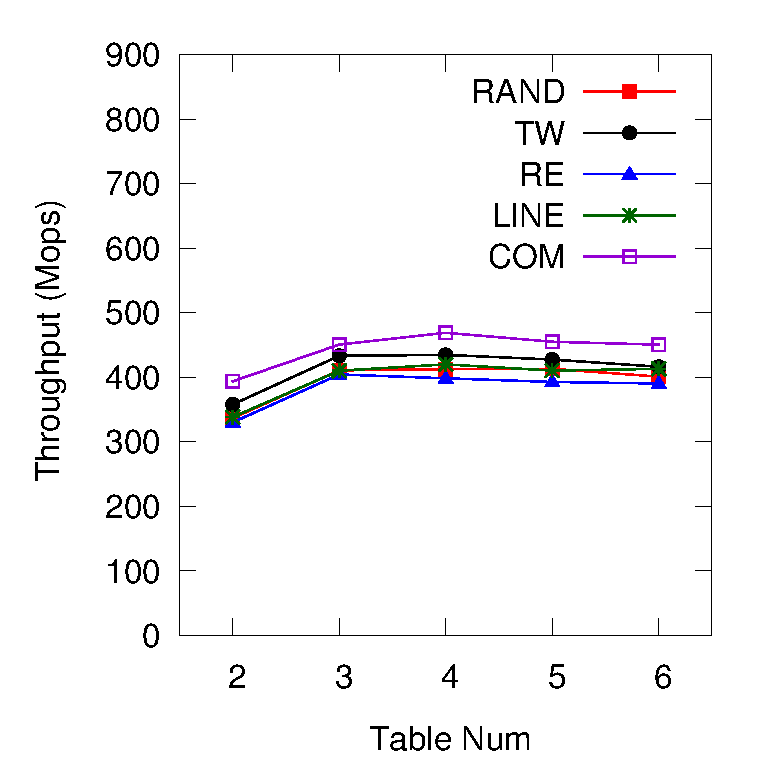
\includegraphics[width=\linewidth]{pic/tunning/tunning-insert.eps}
		\centerline{\formal{insert}}
	\end{minipage}
	\hfill
	\begin{minipage}{0.48\linewidth}\centering
		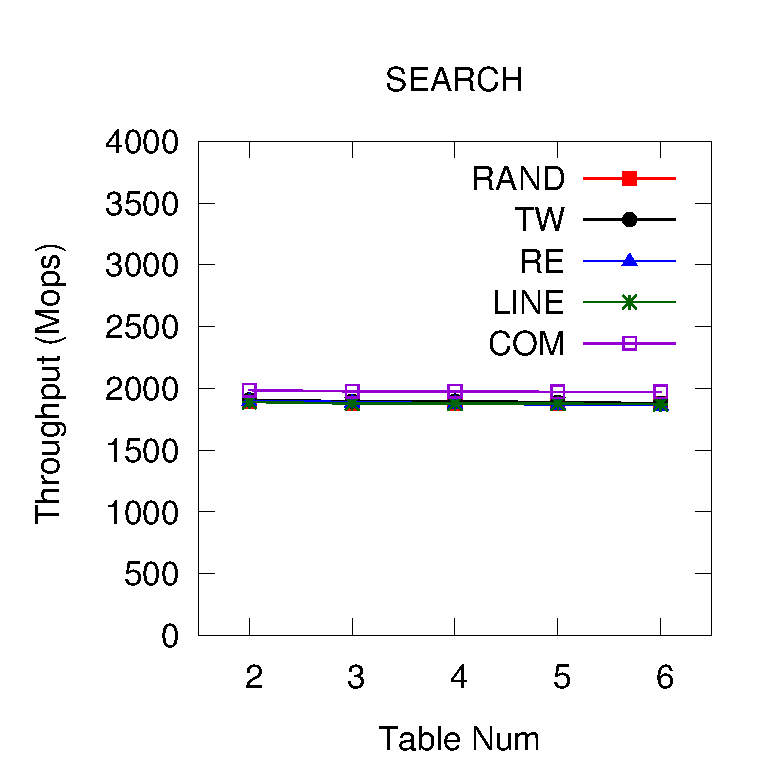
\includegraphics[width=\linewidth]{pic/tunning/tunning-search.eps}
		\centerline{\formal{find}}
	\end{minipage}
	\caption{Throughput of \voter when varying the number of hash tables.}
	\label{fig:vary-table}
\end{figure}
%
\begin{figure}[t]
	\begin{minipage}{0.45\linewidth}\centering
		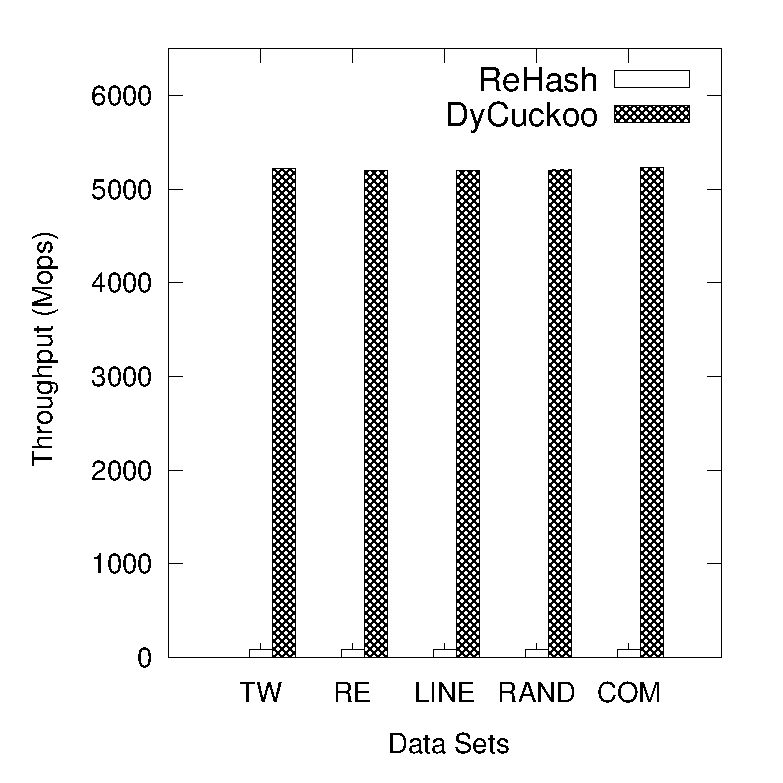
\includegraphics[width=\linewidth]{pic/compare/upsize.eps}
		\centerline{\formal{upsize}}
	\end{minipage}
	\hfill
	\begin{minipage}{0.45\linewidth}\centering
		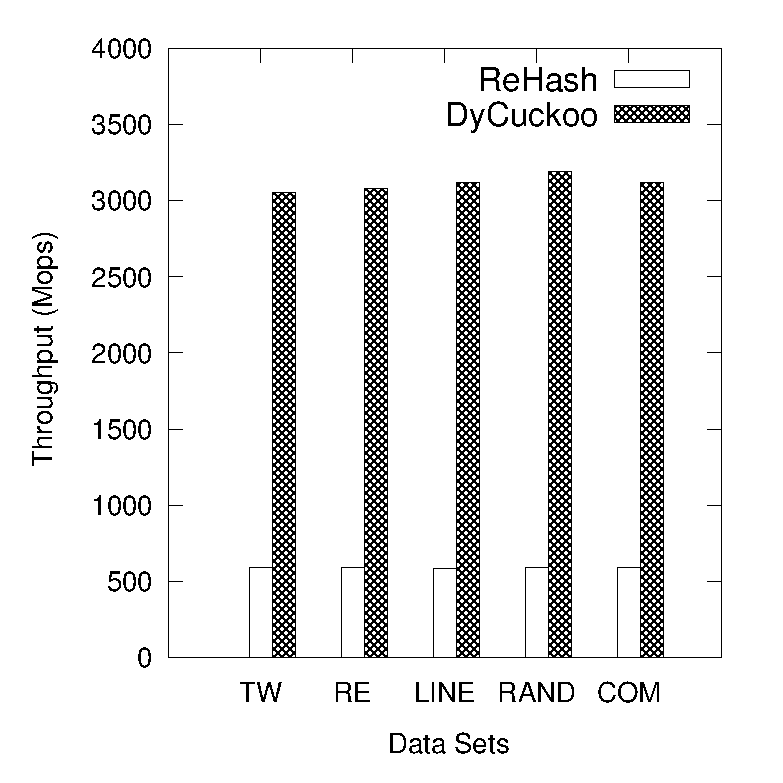
\includegraphics[width=\linewidth]{pic/compare/downsize.eps}
		\centerline{\formal{downsize}}
	\end{minipage}
	\caption{Throughput of subtable resize.}
	\label{fig:resize}
\end{figure}
%
\begin{figure}[t]
	\begin{minipage}{0.48\linewidth}\centering
		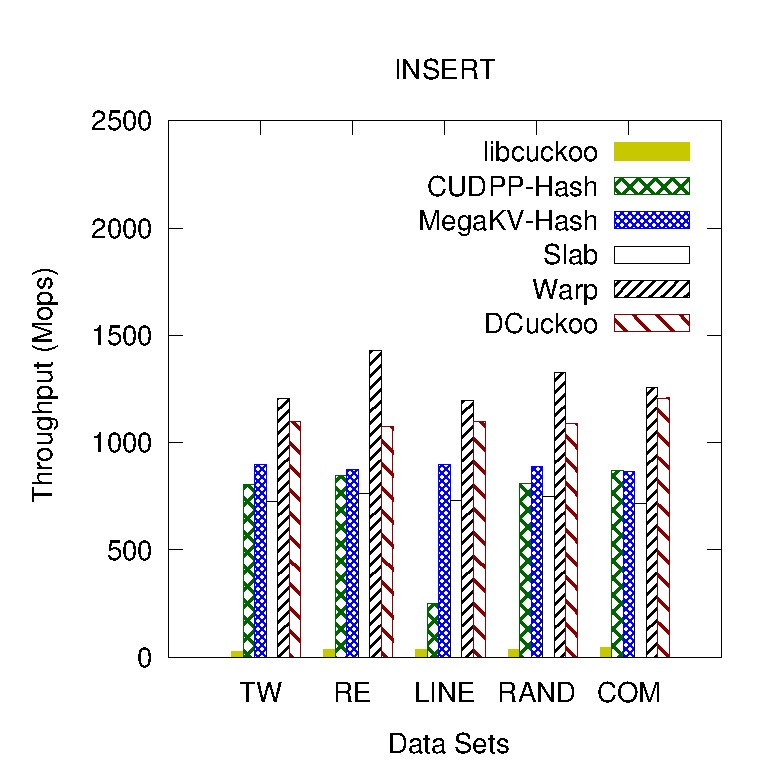
\includegraphics[width=\linewidth]{pic/static/static_insert.eps}
		\centerline{\formal{insert}}
	\end{minipage}
	\hfill
	\begin{minipage}{0.48\linewidth}\centering
		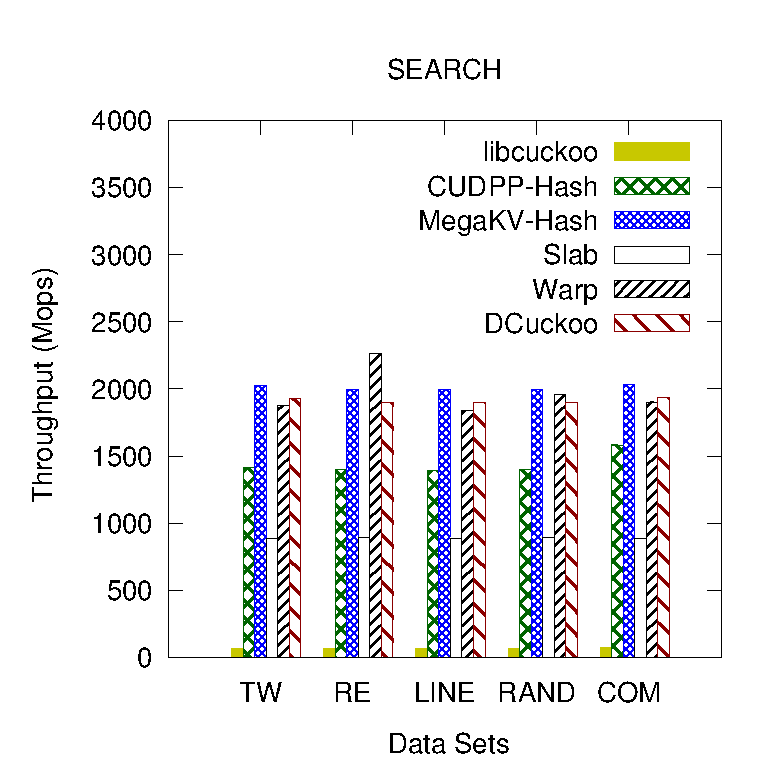
\includegraphics[width=\linewidth]{pic/static/static_search.eps}
		\centerline{\formal{find}}
	\end{minipage}
	\caption{Throughput of all compared approaches under the static setting.}
	\label{fig:static-all}
\end{figure}
%
\begin{figure}[t]
	\begin{minipage}{0.48\linewidth}\centering
		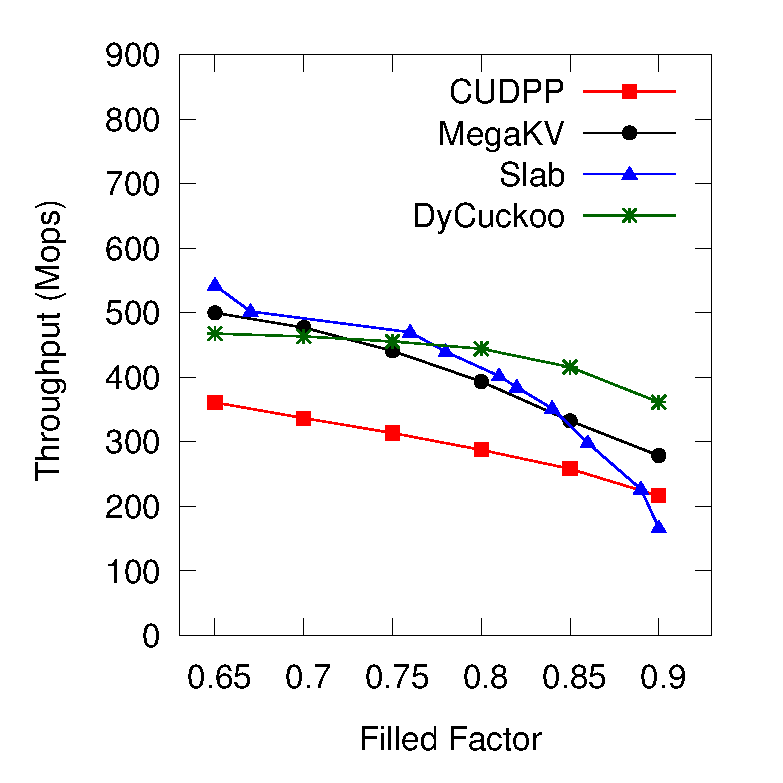
\includegraphics[width=\linewidth]{pic/static-load_factor/insert.eps}
		\centerline{\formal{insert}}
	\end{minipage}
	\hfill
	\begin{minipage}{0.48\linewidth}\centering
		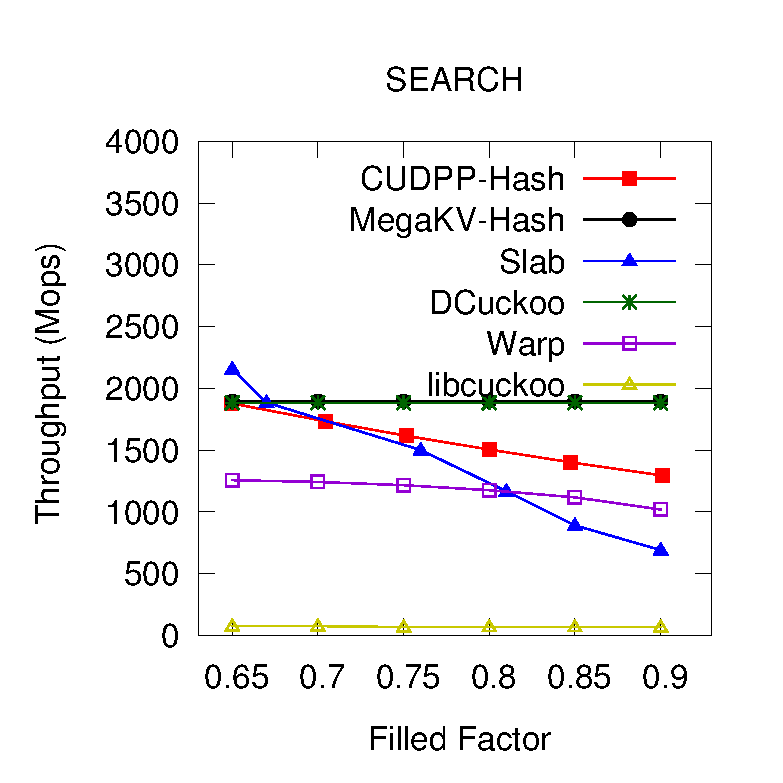
\includegraphics[width=\linewidth]{pic/static-load_factor/search.eps}
		\centerline{\formal{find}}
	\end{minipage}
	\caption{Throughput of all compared approaches for varying the filled factor against the \dsali dataset.\yc{change load factor to filled factor. This figure is not consistent with Figure~\ref{fig:static-filled factor}}}
	\label{fig:static-filled factor}
\end{figure}


\vspace{1mm}\noindent\textbf{Static Hashing Comparison (Section~\ref{sec:exp:static}).}
Under the static setting, we evaluate \formal{insert} and \formal{find} performance among all compared approaches. 
In particular, we insert all KV pairs from the datasets followed by issuing 1 million random search queries. 



%\begin{figure*}[ht]
%	\begin{minipage}{0.3\linewidth}\centering
%		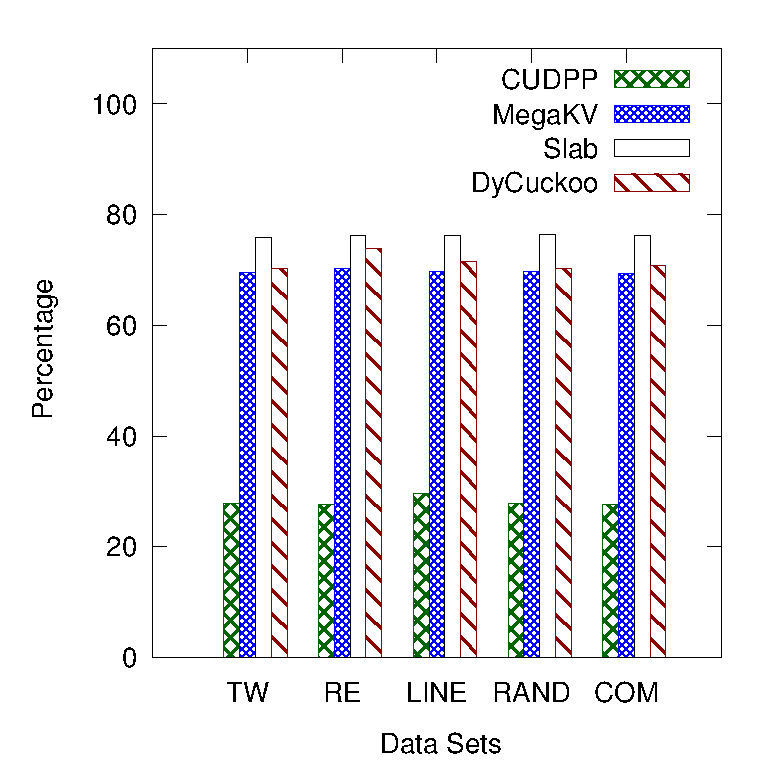
\includegraphics[width=\linewidth]{pic/static-profi/warp.eps}
%		\centerline{Warp Efficiency}
%	\end{minipage}
%	\hfill
%	\begin{minipage}{0.3\linewidth}\centering
%		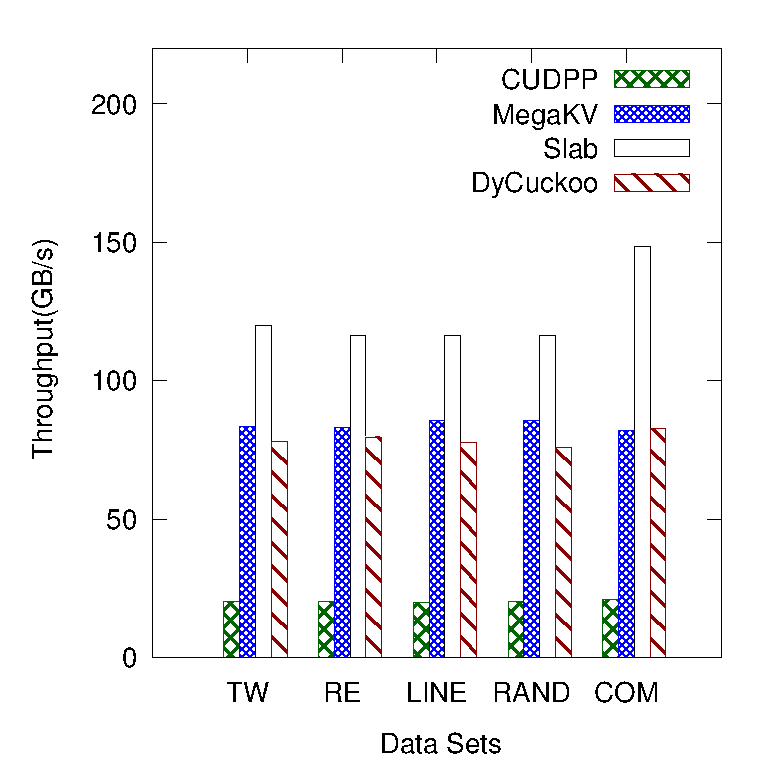
\includegraphics[width=\linewidth]{pic/static-profi/L2-read.eps}
%		\centerline{Cache Utilization}
%	\end{minipage}
%	\hfill
%	\begin{minipage}{0.3\linewidth}\centering
%		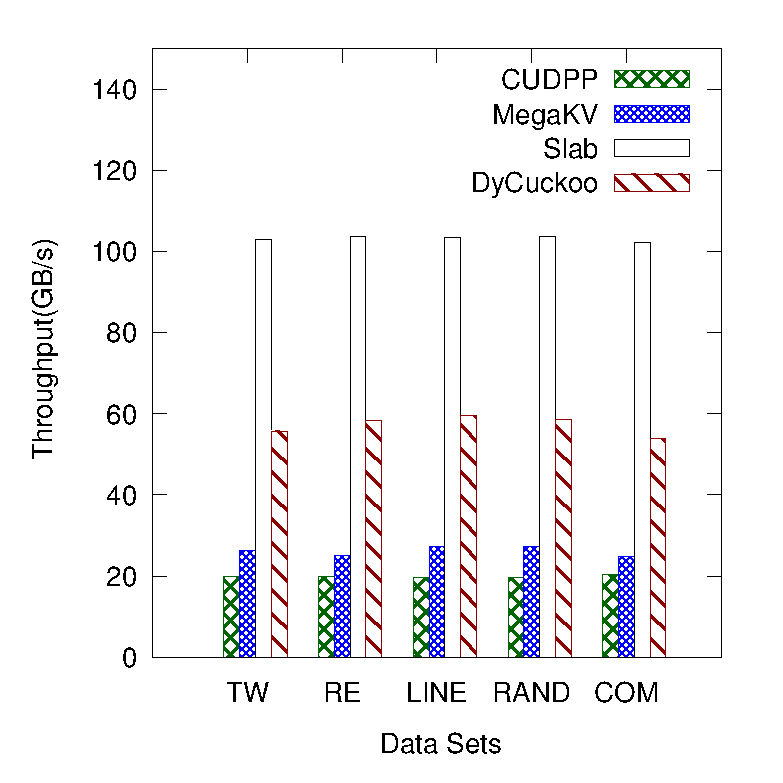
\includegraphics[width=\linewidth]{pic/static-profi/memory-read.eps}
%		\centerline{Memory Bandwidth Utilization}
%	\end{minipage}
%	\caption{GPU profiling results for static hashing comparison.}
%	\label{fig:static:profile}
%\end{figure*}


\vspace{1mm}\noindent\textbf{Dynamic Hashing Comparison (Section~\ref{sec:exp:dynamic}).}
Under the dynamic setting, we generate the workloads by batching the hash table operations. 
We partition the datasets into batches of $1$ million insertions. 
For each batch, we augment $1$ million \formal{find} operations and $1 \cdot r$ million \formal{delete} operations,
where $r$ is a parameter to balance insertions and deletions.
After we exhaust all the batches, we rerun these batches by swapping the \formal{insert} and \formal{delete} operations in each batch. 
We evaluate the performance of all compared approaches except \cudpp as it does not support deletions. 
Since \megakv is a static hash table, we double/half the memory usage followed by rehashing all KV pairs as its resizing strategy, if the corresponding filled factor falls out of the specified range. 
Moreover, if an insertion failure is found for a compared approach, we trigger its resizing strategy.



\vspace{1mm}\noindent\textbf{Parameters.}
We vary the parameters when comparing \voter with the baselines.
$\alpha$ is the lower bound on the filled factor $\theta$ for all compared approaches,
whereas $\beta$ is the respective upper bound.
$r$ is the ratio of insertions over deletions in a processing batch. 
The settings of the aforementioned parameters could be found in Table~\ref{tbl:parameters}. For all experiments, we use \emph{million operations/seconds} (Mops) to measure the performance of all compared approaches.

\vspace{1mm}\noindent\textbf{Experiment Environment.}
We conduct all experiments on an Intel Xeon E5-2620 Server equipped with NVIDIA GeForce GTX 1080.The GTX 1080 is built on Pascal architecture with 20 SMs and 128 SPs per SM. The GTX 1080 has 8 GB of GDDR5 memory. Evaluations are performed using CUDA 8.0 on Ubuntu 16.04.3. The optimization level (-O3) is applied for compiling all programs.





\subsection{Sensitivity Analysis}\label{sec:exp:tune}

\vspace{1mm}
\noindent\textbf{Vary the number of tables.}
A key parameter that affects the performance of \voter is the number of hash table chosen. For the static scenario, we present the throughput performance of \formal{insert} and \formal{find} for varying number of hash tables in Figure~\ref{fig:vary-table}, while fixing the memory space of the entire structure to ensure the default filled factor $\theta$. 
The throughput of \formal{insert} increases with more hash tables, since there are more alternative locations for relocating a KV pair. However, the marginal improvement drops for a larger number of hash tables. Furthermore, the throughput of \formal{find} remains constant for additional hash tables incorporated as the two-layer cuckoo hashing guarantees at most two look ups for \formal{find}. In the remaining part of this section, we fix the number of hash tables to be $4$.

\vspace{1mm}
\noindent\textbf{Resizing analysis.}
To validate the effectiveness of our resizing strategy proposed in Section~\ref{sec:dyn}, we compare it with rehashing. 
For evaluating upsizing, we initialize \voter with all the data and the filled factor as the default upper bound $85\%$. Then, we perform one time upsizing, i.e., upsize one subtable, and compare our resizing strategy against rehashing all the entries in the subtable with Algorithm~\ref{algo:insert}.
For evaluating downsizing, the setup is a mirror image of upsizing evaluation with an initializing filled factor as the default lower bound $30\%$. 
The throughputs are reported in Figure~\ref{fig:resize}. 
The throughput of rehashing for the upsizing scenario is severely limited, since the remaining subtables not being upsized are almost filled and inserting KV pairs resulting frequent evictions.  
In comparison, the downsizing throughput of rehashing is significantly faster due to a low filled ratio.
Our resizing strategy achieves compelling speedups over rehashing. Besides, it only locks the subtable being resized and supports concurrent updates for the remaining subtables. 


\subsection{Static Hashing Comparison}\label{sec:exp:static}

\vspace{1mm}\noindent\textbf{Throughput Analysis.} In Figure~\ref{fig:static-all}, we present the throughput of all compared approaches over all datasets under the default setting.
Both \megakv and \cudpp are cuckoo hash approaches but \megakv shows better performance due to its bucket structure, which fully utilizes the cache line for optimizing random access performance.
\megakv and \slab are competitive against each other
while our proposed \voter demonstrates the best throughput for insertion. This is because \voter can reallocate KV pairs to more buckets among $d$ hash tables whereas \megakv can only choose one of two buckets for a KV pair, which causes \megakv to have more evictions. For \formal{find}, \megakv shows the best performance since it simply checks two buckets for locating a KV pair.
Although \voter also checks two buckets, it has slightly inferior performance than \megakv as \voter employs another layer of hashing that adds cost to the overall performance. As \slab employs a chaining approach, it requires more random accesses to locate a KV pair along the chain when a high filled factor is required. Hence, \slab has inferior performance than those of \megakv and \voter.
The experiments show that \voter is competitive even for the static scenario.

\vspace{1mm}\noindent\textbf{Varying filled factor $\theta$.}
We vary the filled factor $\theta$ and show the performance of all compared approaches against the \dsali dataset. The other datasets show similar trend and thus we omit the results in the paper.
For cuckoo hash approaches, i.e., \cudpp, \megakv and \voter, 
the insertion performance slightly degrades for a higher filled factor. \voter shows better stability for insertion as it employs the two-layer hashing approach which allows it to reallocate KV pairs efficiently even when the hash table is almost filled ($\theta=90\%$).
As cuckoo hash approaches only require constant lookups for \formal{find}, the performance is not affected by the filled factor.
For \slab, the performance of both \formal{insert} and \formal{find} is dramatically affected by the filled factor. When $\theta=90\%$, \voter outperforms \slab by over 2.5x and 3x for \formal{insert} and \formal{find} respectively.


%\vspace{1mm}\noindent\textbf{GPU Profiling.} To further study the behavior of the approaches, we present three types of profiling results for all \formal{insert} GPU kernels in Figure~\ref{fig:static:profile}.
%For \emph{warp efficiency}, \voter maintains a stable rate at around 70\%, which is significantly higher than the other two cuckoo hash approaches: \megakv and \cudpp.  
%We attribute this phenomenon to the voter mechanism proposed in Section~\ref{sec:vot:con}, which yields better overall load balancing. 
%\linear could achieve higher warp efficiency than \voter, but is very volatile across different datasets. This is because each \formal{insert} in \linear may require scanning varying number of hash values for distinct data distributions. 
%For example, in the \dsali dataset, its warp efficiency drops below 40\% since \dsali contains more duplicated keys than other datasets. 

%Looking at \emph{cache} and \emph{memory bandwidth} profiling results, \megakv and \voter demonstrate better utilization as they employ the bucket mechanism.
%As \voter always needs to use atomicCAS to lock a bucket before accessing it, its utilization is inferior than that of \megakv due to the additional IO when inserting a KV pair to a bucket. In addition, atomicCAS is less efficient than atomicExch as it involves more workload per operation (see Table~\ref{fig:atomic}). Nevertheless, implementations based on atomicExch only supports KV pair with 64 bits, whereas adopting atomicCAS in \voter can support arbitrary length as we lock the bucket for exclusive update.
%It is also noted that, even though \megakv has great cache utilization due to the use of atomicExch accessing buckets directly, the overall performance is eventually bounded by device memory IOs. 

%In summary, under the static environment, \voter achieves competitive efficiency against the compared GPU baselines. Moreover, although \voter does not deliver the best performance over existing approaches, it has very low insertion failure rate and supports more general hash tables.


%
\begin{figure*}[htp]
	\begin{minipage}{0.19\linewidth}\centering
		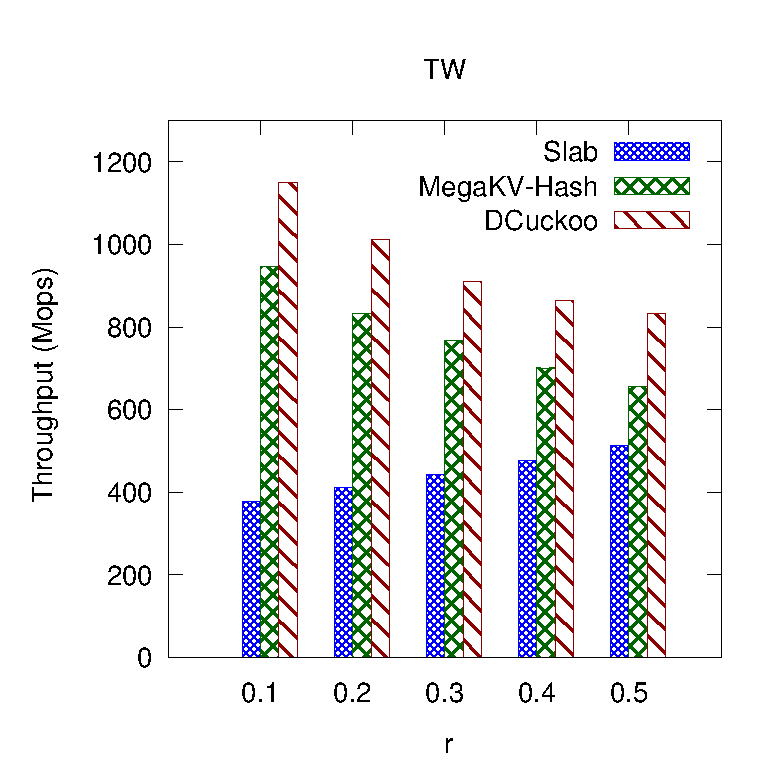
\includegraphics[width=\linewidth]{pic/dynamic/r/dynamic_twitter.eps}
		\centerline{\dstwitter}
	\end{minipage}
	\begin{minipage}{0.19\linewidth}\centering
		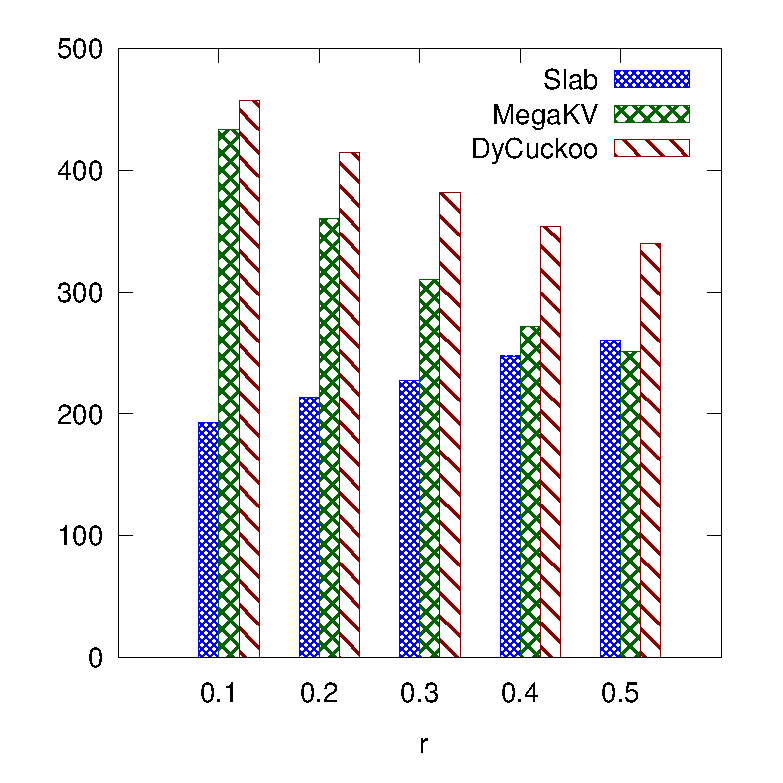
\includegraphics[width=\linewidth]{pic/dynamic/r/dynamic_reddit.eps}
		\centerline{\dsreddit}
	\end{minipage}
	\begin{minipage}{0.19\linewidth}\centering
		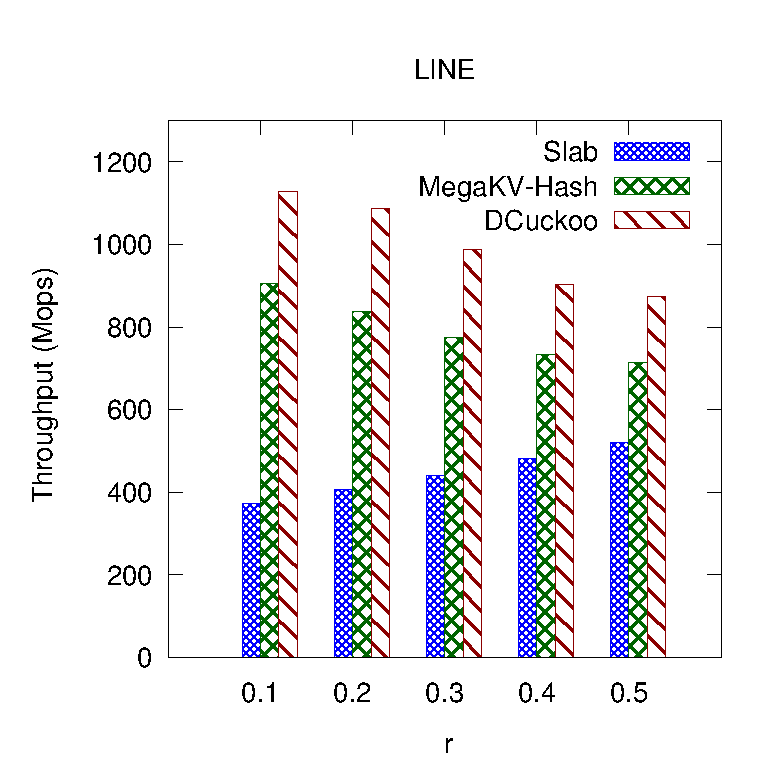
\includegraphics[width=\linewidth]{pic/dynamic/r/dynamic_tpch.eps}
		\centerline{\dstpch}
	\end{minipage}
	\begin{minipage}{0.19\linewidth}\centering
		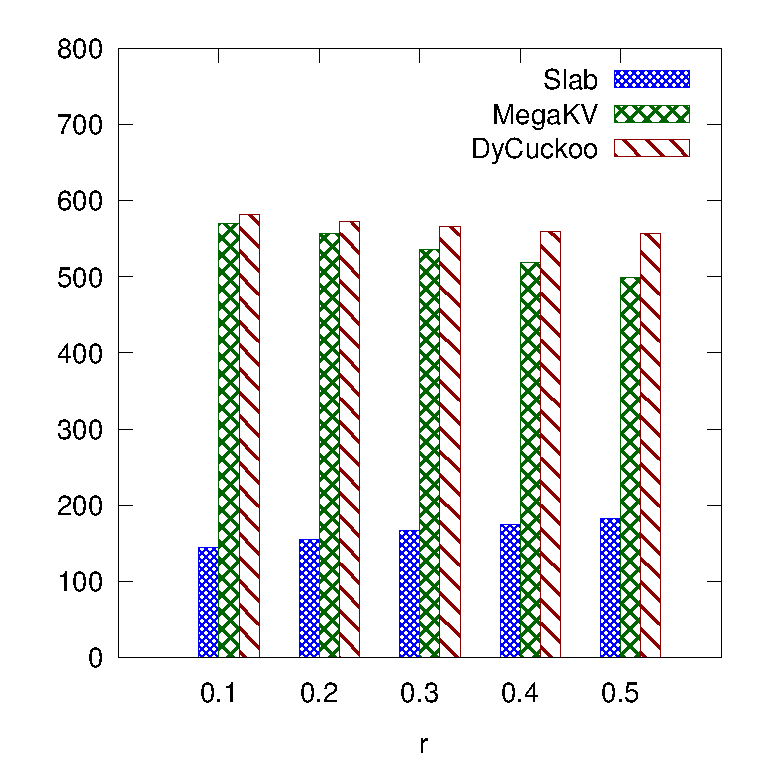
\includegraphics[width=\linewidth]{pic/dynamic/r/dynamic_ali.eps}
		\centerline{\dsali}
	\end{minipage}
	\begin{minipage}{0.19\linewidth}\centering
		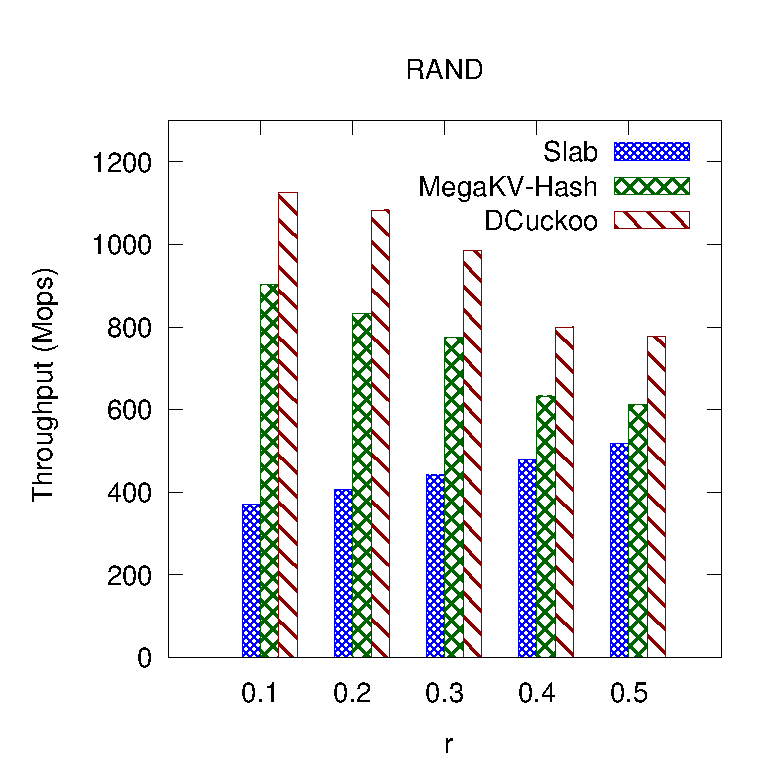
\includegraphics[width=\linewidth]{pic/dynamic/r/dynamic_random.eps}
		\centerline{\dsrandom}
	\end{minipage}
	\caption{Run time for varying $r$.}
	\label{fig:vary-r-time}
\end{figure*}
%
\begin{figure*}[htp]
	\begin{minipage}{0.19\linewidth}\centering
		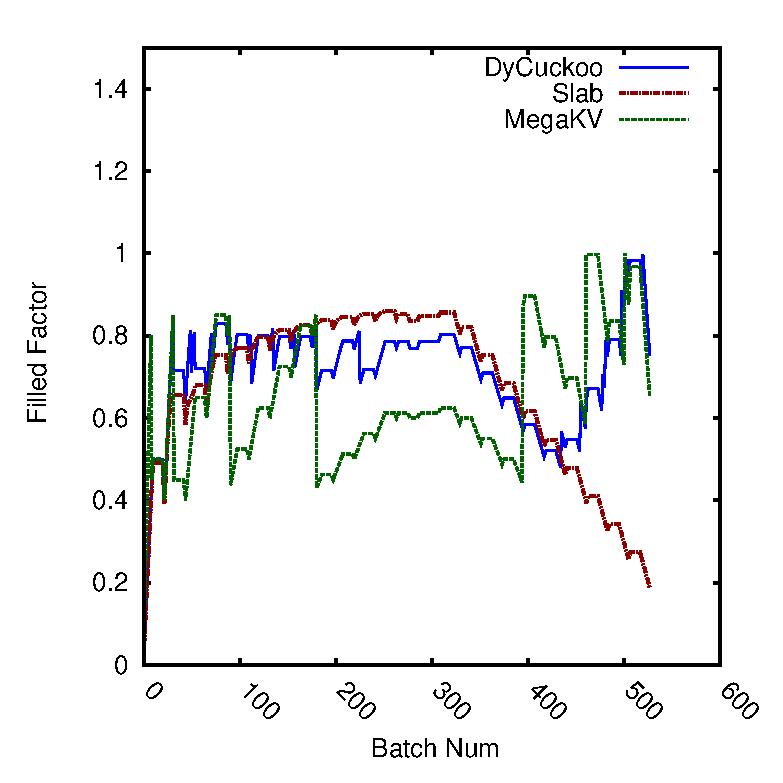
\includegraphics[width=\linewidth]{pic/dynamic-load_factor/twitter/batch_LoadFactor-2.eps}
		\centerline{\dstwitter}
	\end{minipage}
	\begin{minipage}{0.19\linewidth}\centering
		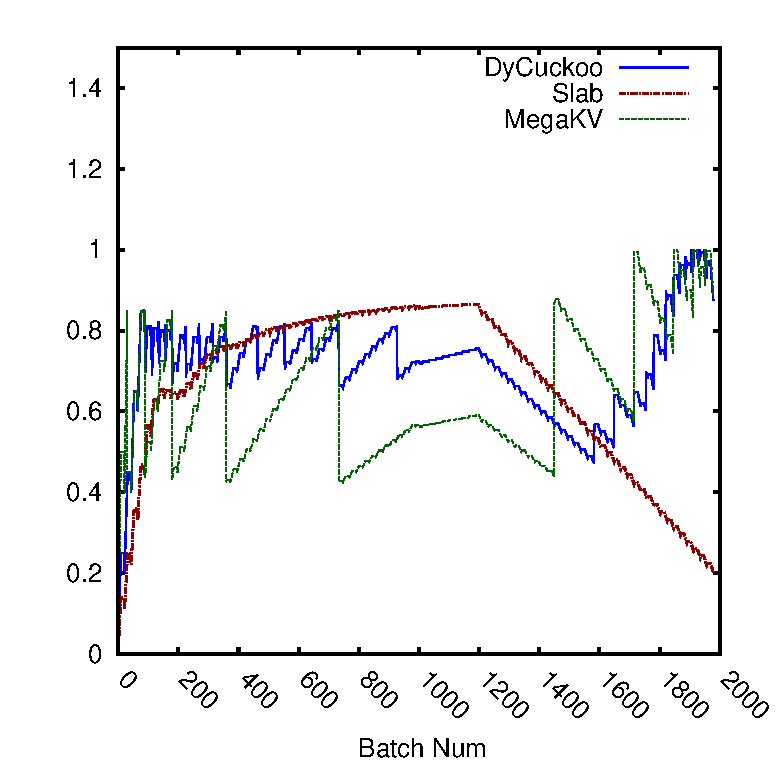
\includegraphics[width=\linewidth]{pic/dynamic-load_factor/reddit/batch_LoadFactor-2.eps}
		\centerline{\dsreddit}
	\end{minipage}
	\begin{minipage}{0.19\linewidth}\centering
		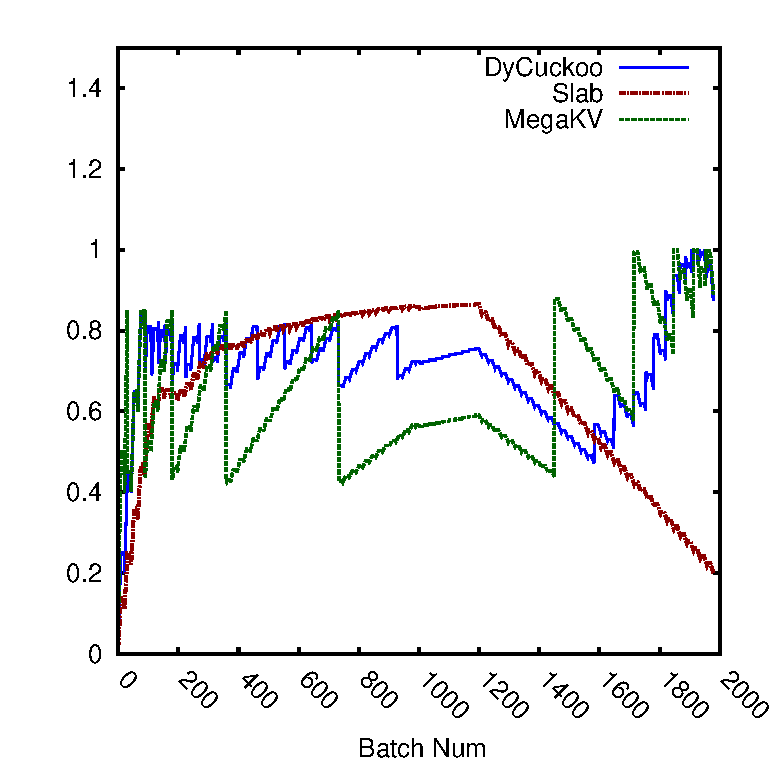
\includegraphics[width=\linewidth]{pic/dynamic-load_factor/tpch/batch_LoadFactor-2.eps}
		\centerline{\dstpch}
	\end{minipage}
	\begin{minipage}{0.19\linewidth}\centering
		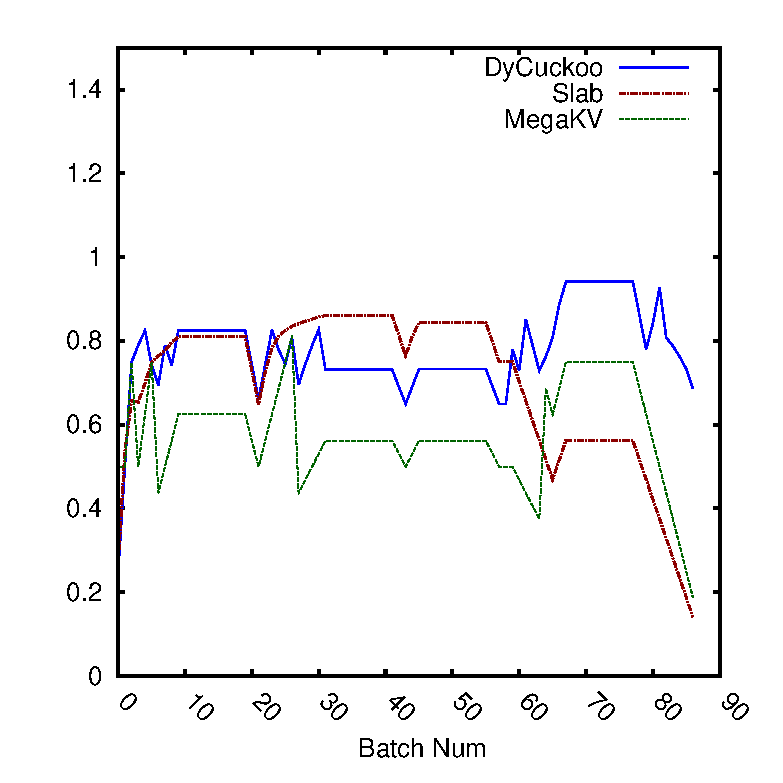
\includegraphics[width=\linewidth]{pic/dynamic-load_factor/ali/batch_LoadFactor-2.eps}
		\centerline{\dsali}
	\end{minipage}
	\begin{minipage}{0.19\linewidth}\centering
		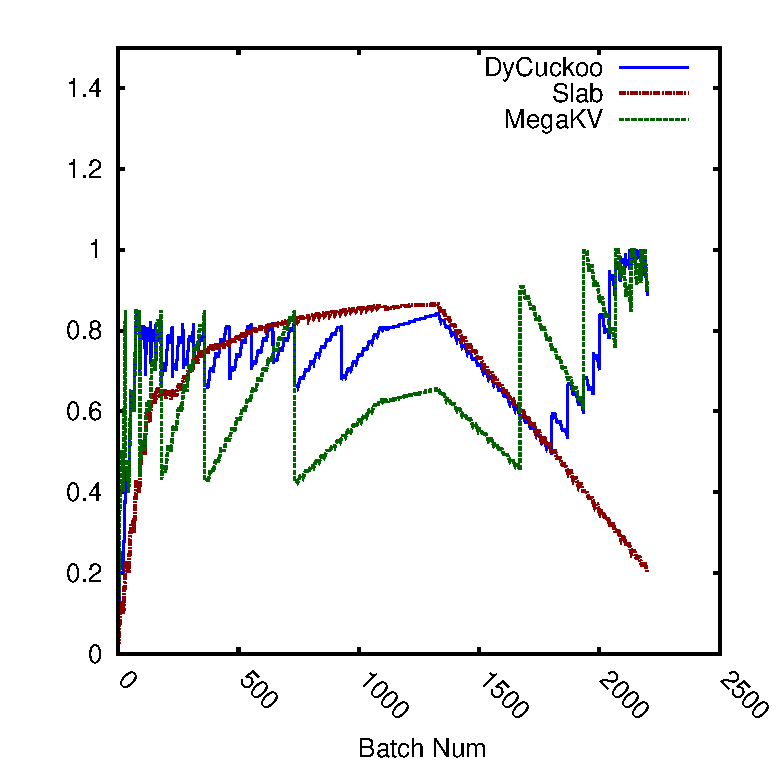
\includegraphics[width=\linewidth]{pic/dynamic-load_factor/random/batch_LoadFactor-2.eps}
		\centerline{\dsrandom}
	\end{minipage}
	\caption{Tracking the filled factor.\yc{change load factor to filled factor.}}
	\label{fig:track-stability}
\end{figure*}





\subsection{Dynamic Hashing Comparison}\label{sec:exp:dynamic}


\vspace{1mm}\noindent\textbf{Varying insert vs. delete ratio $r$.}
In Figure~\ref{fig:vary-r-time}, we report the results for varying the ratio $r$ of number of deletions over number of insertions.
We have an interesting observation that, for a larger $r$, the performance of \voter and \megakv degrades whereas that of \slab improves. As a larger $r$ indicates more deletions, resizing operations are more frequently invoked for \voter and \megakv. In contrast, more deletions leads to additional vacant spaces for \slab as it only symbolically marks a deleted KV pair. Insertions are processed more efficiently for \slab since the inserted KV pairs can overwrite the symbolically deleted ones. Hence, \slab utilizes more GPU device memory than \voter and \megakv. However, symbolic deletions cannot guarantee a bounded filled factor and may lead to arbitrary bad memory efficiency, which will be discussed with more experimental results later in this section.
\voter shows the best overall performance. Furthermore, the throughput margin between \voter and \megakv grows for a larger $r$. 
As aforementioned, larger $r$ triggers more resizing operations, where \voter is more efficient to handle. 

%\linear and \megakv remains inefficient as they incur expensive overheads of resizing. An interesting observation for \linear and \megakv is that there exists a sweet spot where the resizing cost is the minimal.
%It is because the workload composition of insertions and deletions should be just right so that it does not trigger unnecessary upsizings or downsizings. However, in reality, the workloads could vary significantly and existing methods cannot be easily adapted while maintaining guaranteed filled factor. This has again validated the effectiveness of \voter against dynamic workloads.


\vspace{1mm}\noindent\textbf{Performance stability.}
We evaluate the performance stability of the compared approaches in Figure~\ref{fig:track-stability}. 
In particular, we track the filled factor after processing each batch.
\slab shows good stability in terms of memory usage for the starting phases. 


\vspace{1mm}\noindent\textbf{Varying the batch size.}
We have also varied the size of each processing batch. The results are reported in Figure~\ref{fig:vary-batch-size}. \voter remains the most efficient method over \linear and \megakv. It is not surprised to find that the performance of \linear and \megakv is the worst for the smallest batch size, since a fine-grained processing batch triggers additional resizing for \linear and \megakv. 




\begin{figure*}[htp]
	\begin{minipage}{0.19\linewidth}\centering
		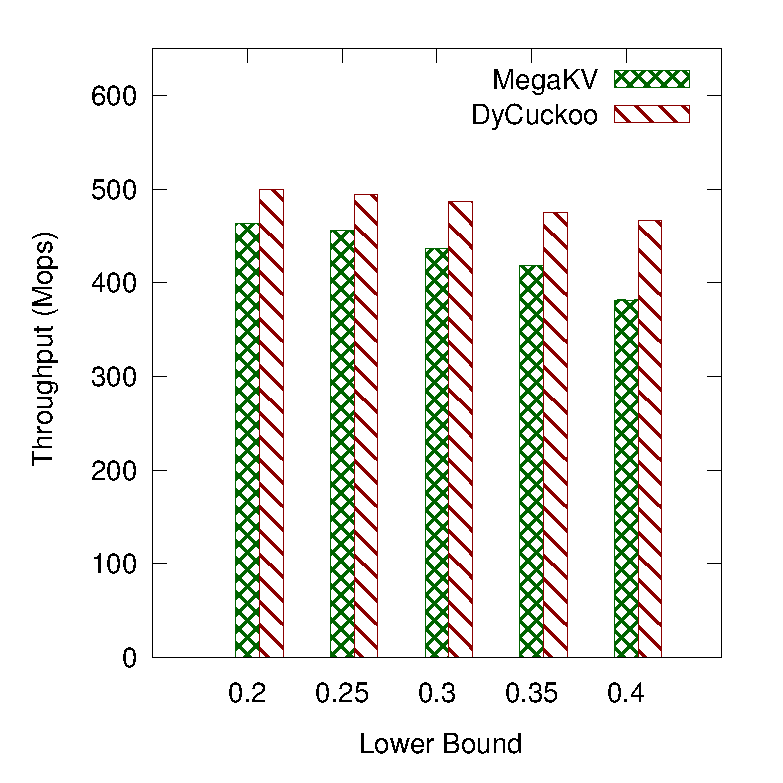
\includegraphics[width=\linewidth]{pic/dynamic/lower/dynamic_twitter.eps}
		\centerline{\dstwitter}
	\end{minipage}
	\begin{minipage}{0.19\linewidth}\centering
		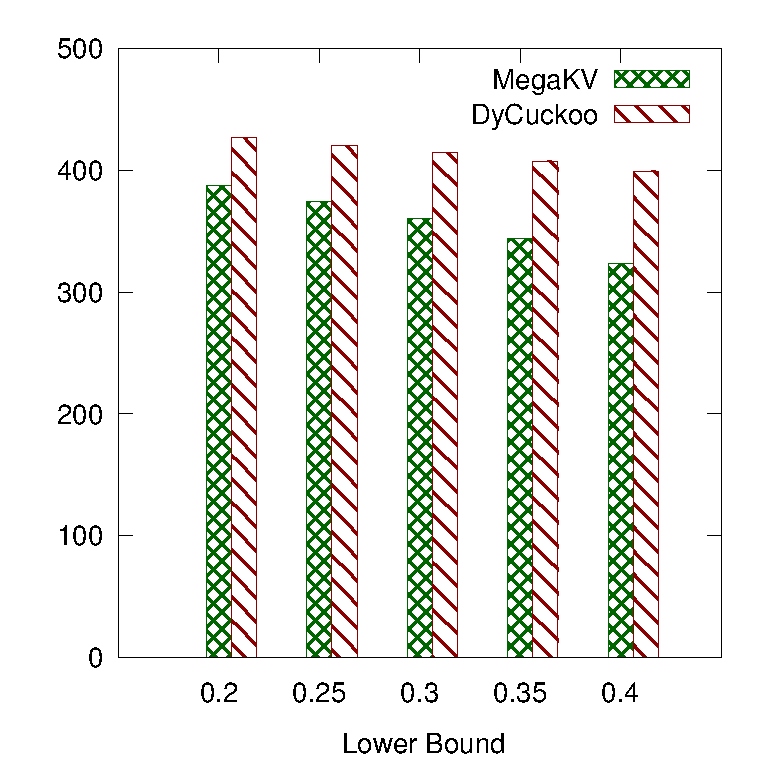
\includegraphics[width=\linewidth]{pic/dynamic/lower/dynamic_reddit.eps}
		\centerline{\dsreddit}
	\end{minipage}
	\begin{minipage}{0.19\linewidth}\centering
		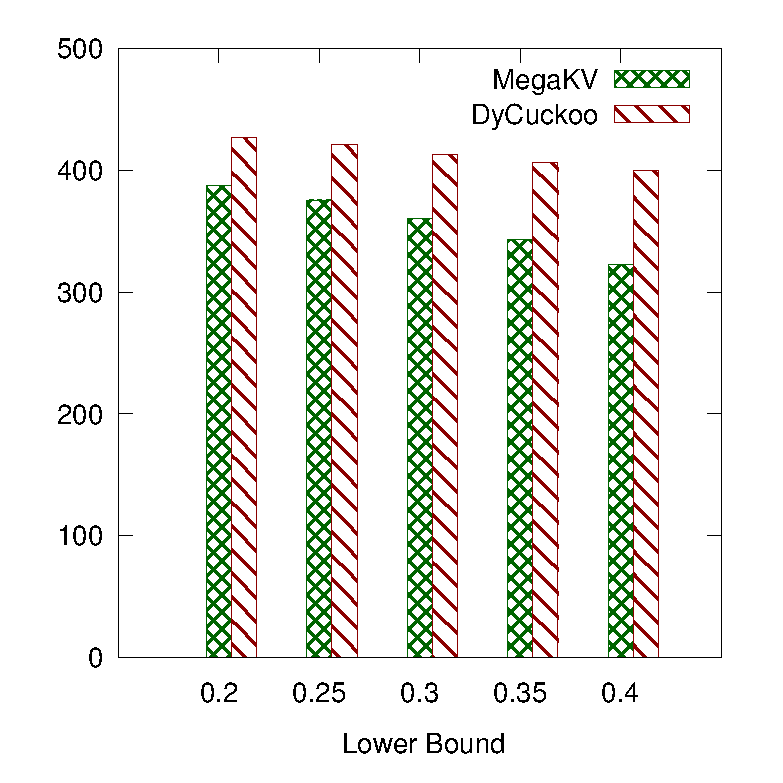
\includegraphics[width=\linewidth]{pic/dynamic/lower/dynamic_tpch.eps}
		\centerline{\dstpch}
	\end{minipage}
	\begin{minipage}{0.19\linewidth}\centering
		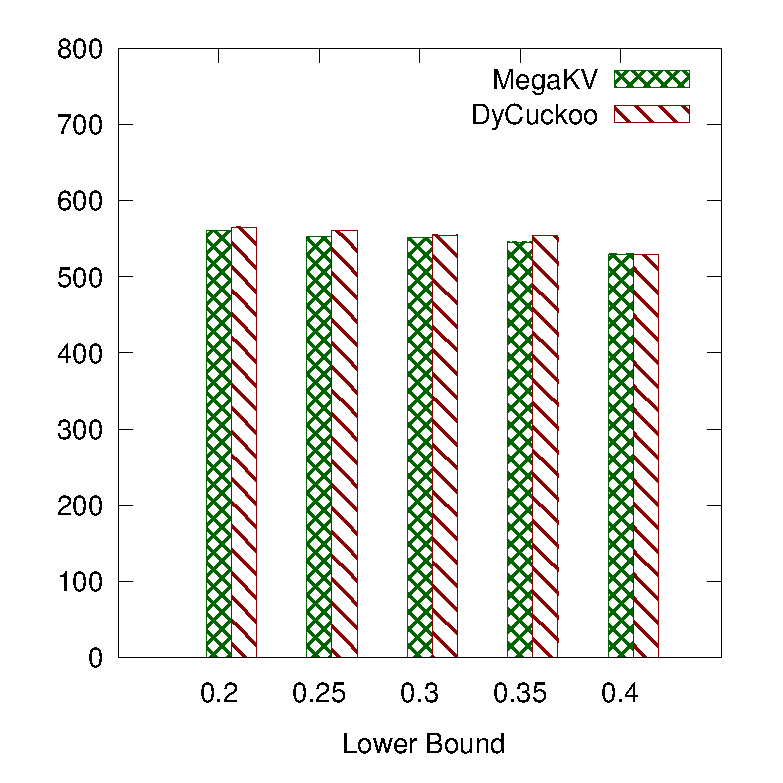
\includegraphics[width=\linewidth]{pic/dynamic/lower/dynamic_ali.eps}
		\centerline{\dsali}
	\end{minipage}
	\begin{minipage}{0.19\linewidth}\centering
		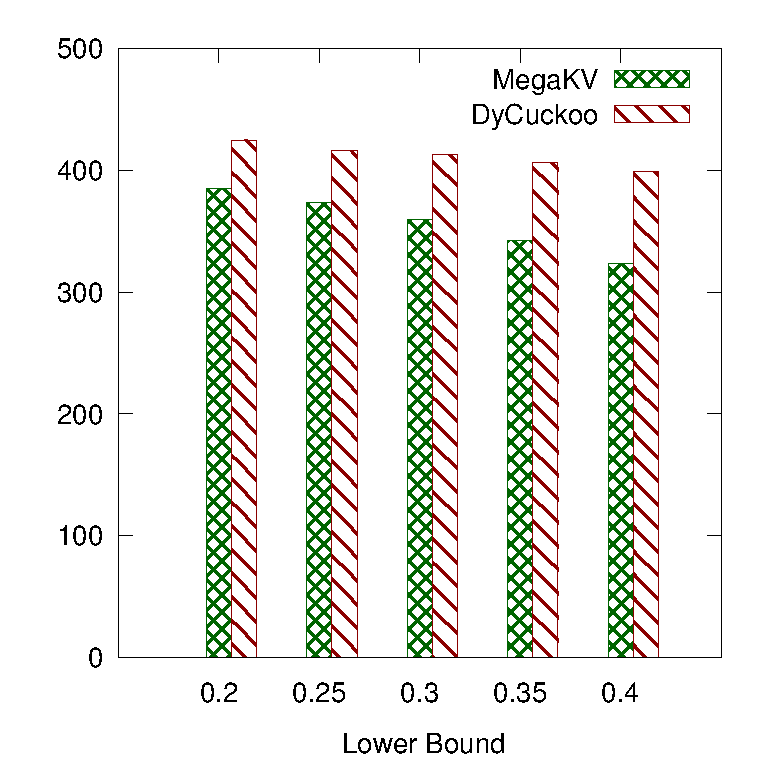
\includegraphics[width=\linewidth]{pic/dynamic/lower/dynamic_random.eps}
		\centerline{\dsrandom}
	\end{minipage}
	\caption{Run time for varying $\alpha$ .}
	\label{fig:vary-lower-time}
\end{figure*}

\begin{figure*}[htp]
	\begin{minipage}{0.19\linewidth}\centering
		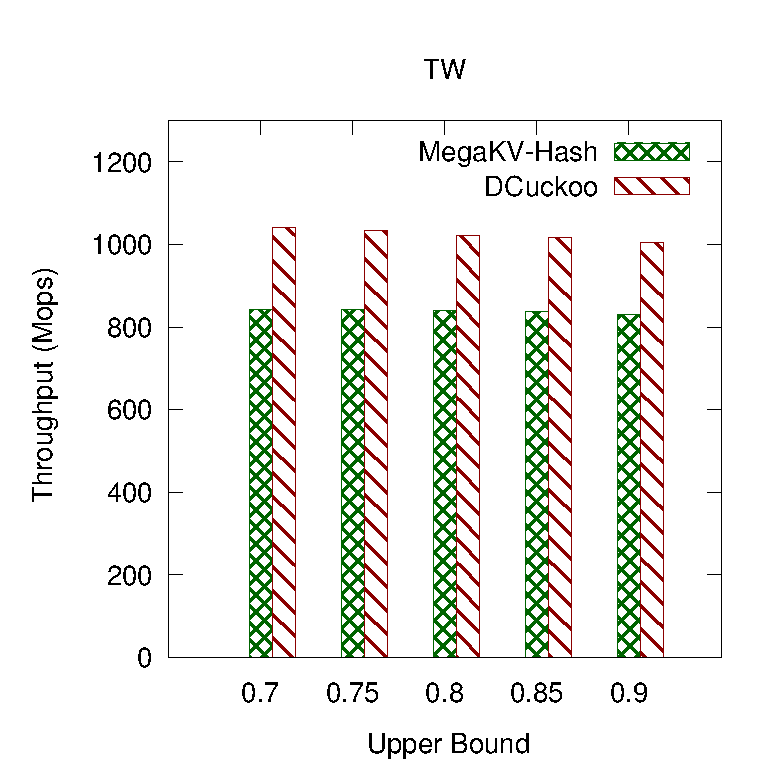
\includegraphics[width=\linewidth]{pic/dynamic/upper/dynamic_twitter.eps}
		\centerline{\dstwitter}
	\end{minipage}
	\begin{minipage}{0.19\linewidth}\centering
		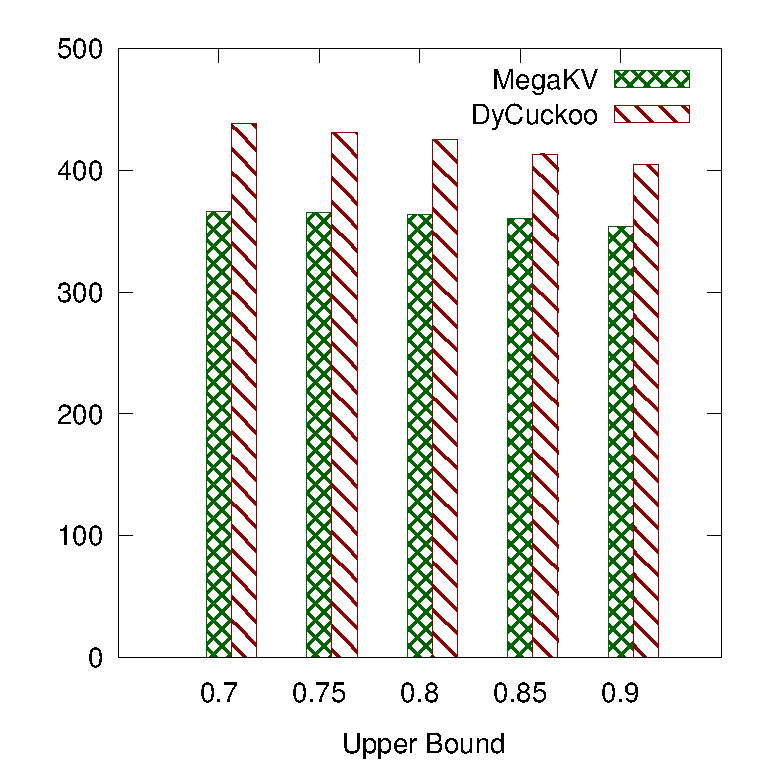
\includegraphics[width=\linewidth]{pic/dynamic/upper/dynamic_reddit.eps}
		\centerline{\dsreddit}
	\end{minipage}
	\begin{minipage}{0.19\linewidth}\centering
		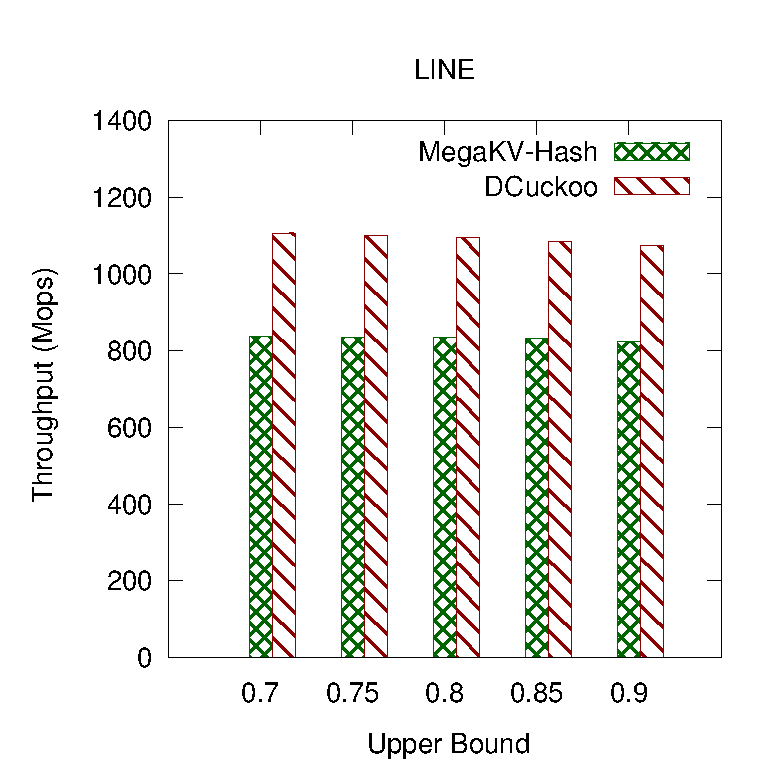
\includegraphics[width=\linewidth]{pic/dynamic/upper/dynamic_tpch.eps}
		\centerline{\dstpch}
	\end{minipage}
	\begin{minipage}{0.19\linewidth}\centering
		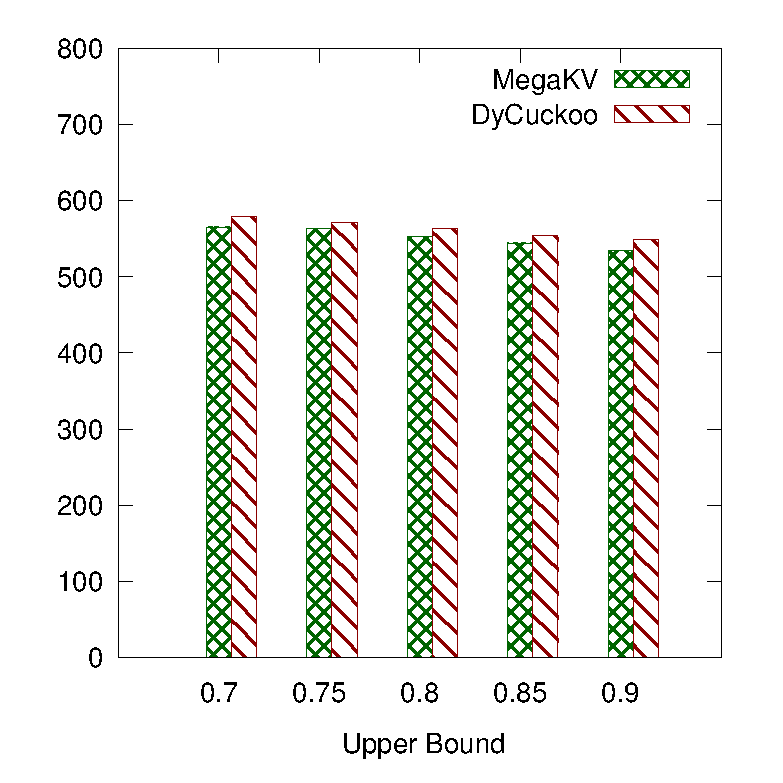
\includegraphics[width=\linewidth]{pic/dynamic/upper/dynamic_ali.eps}
		\centerline{\dsali}
	\end{minipage}
	\begin{minipage}{0.19\linewidth}\centering
		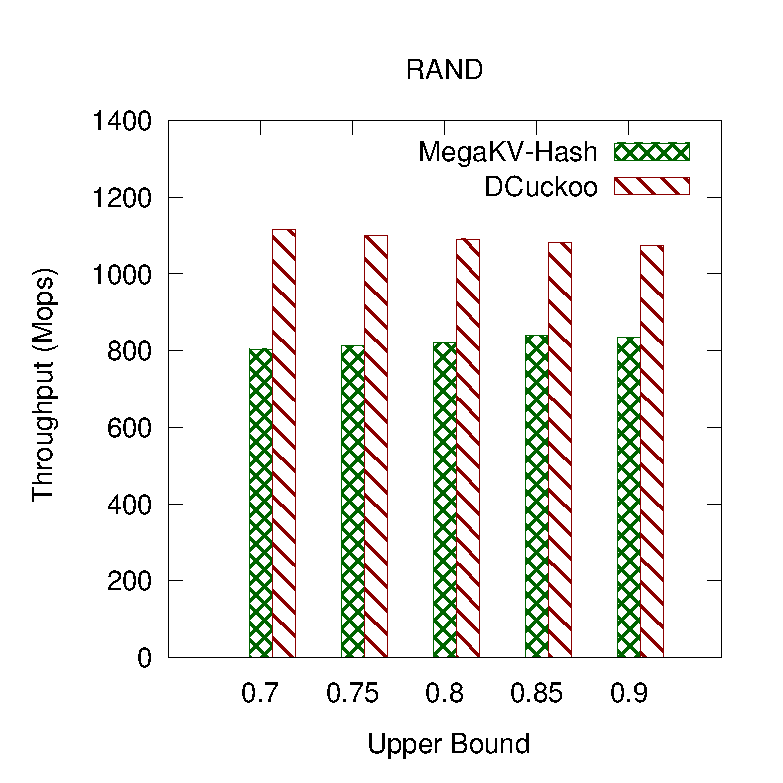
\includegraphics[width=\linewidth]{pic/dynamic/upper/dynamic_random.eps}
		\centerline{\dsrandom}
	\end{minipage}
	\caption{Run time for varying $\beta$ .}
	\label{fig:vary-upper-time}
\end{figure*}

\vspace{1mm}\noindent\textbf{Varying the filled factor lower bound $\alpha$.}
We vary the lower bound of the filled factor and report the results in Figure~\ref{fig:vary-alpha-time}. 
The performance is measured by the total running time for processing all batches described in Section~\ref{sec:exp:setup}. Furthermore, we indicate the time taken for all components involved in the processing: \formal{insert}, \formal{find}, \formal{delete} and \formal{resize}. Apparently, the resizing strategy adopted by \linear and \megakv incur significant overhead. Such overhead grows dramatically for a higher $\alpha$ since the number of downsizings are executed. It is noted that the impact of resizing is the more significant for \megakv than \linear. We interpret the phenomenon as the following.
\megakv has a higher insertion failure rate than that of \linear (see Table~\ref{tab:fail:tw}-\ref{tab:fail:com}). Thus, \megakv triggers more upsizings leading to a lower filled ratio when resized. As each processing batch contains deletions, \megakv is prone to downsize when the filled factor falls below $\alpha$ after deletions materialize.
The overhead of repeated resizings severely degrades the performance of \megakv, for the major reason of maintaining the filled factor above $\alpha$. 
The only exception is where $\alpha$ is very small (i.e., $\alpha=0.25$) and \megakv does not need to perform downsizing regularly. However, small $\alpha$ means the hash table is mostly empty and thus wastes GPU memory resources.
In contrast, \voter achieves significant speedups over \linear and \megakv (up to 6.62 and 5.05 faster respectively under the default setting). 
\voter can support even larger $\alpha$ (i.e., $\beta\cdot\frac{d}{d+1}$) but we omit the results since the baselines cannot deliver reasonable performance beyond $\alpha > 0.5$.
There are two reasons behind why \voter's performance. First, \voter has low failure rate and thus avoids unnecessary resizing operations. Second, \voter employs the resizing strategy (proposed in Section~\ref{sec:dyn}) by only relocating the entries in one subtable efficiently. 
Compared with time taken by \formal{insert}, \formal{delete} and \formal{find}, the cost of \formal{resize} for \voter is almost negligible.



\vspace{1mm}\noindent\textbf{Varying the filled factor upper bound $\beta$.}
The results for varying $\beta$ is reported in Figure~\ref{fig:vary-beta}. 
It is interesting to see that the upper bound does not significantly affect the overall performance for all methods. 
For \linear and \megakv, it is very hard for them to achieve high filled factor since upsizing will be triggered once there are failed insertions.
Although \voter also incurs insertion failure, such cases only occur for filled factor beyond $0.9$ and thus the resizing operations are rarely invoked for the sake of handling failed insertions. 
For \voter, it is noted that there is a slight increasing trend for a larger $\beta$, especially in \dsreddit and \dsrandom datasets. 
The increase is mostly attributed to the additional processing workload of the insertions at a higher filled factor, rather than the resizing cost. 







